% ----- ab hier eigentlicher Inhalt -------------------------------------------

\section[Intro]{Beispiel: C}
\subsection*{}
\begin{frame}
	\frametitle{Sprachdefinition von C}
	\begin{block}{Addition}
		Mithilfe der BNF bzw. EBNF, einer erweiterten Schreibweise von Kontextfreien Grammatiken lässt sich z.B. die Syntax von Programmiersprachen darstellen.
	\end{block}
\end{frame}

\begin{frame}
	\frametitle{Sprachdefinition von C}
	\begin{block}{Addition}
		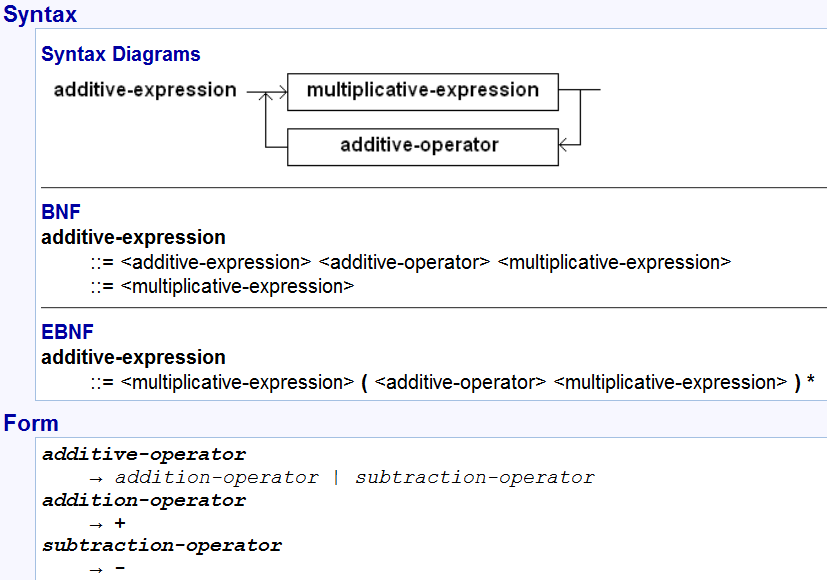
\includegraphics[width=0.8\textwidth]{src/Syntax_Addition_C}
		
	\end{block}
\end{frame}

%diesmal keine, lieber  ein tafelbeispiel oder sowas, pseudocode eignet sich schlecht für ja/nein fragen